% $Header: /cvsroot/latex-beamer/latex-beamer/solutions/generic-talks/generic-ornate-15min-45min.en.tex,v 1.5 2007/01/28 20:48:23 tantau Exp $

% This file is a solution template for:

% - Giving a talk on some subject.
% - The talk is between 15min and 45min long.
% - Style is ornate.



% Copyright 2004 by Till Tantau <tantau@users.sourceforge.net>.
%
% In principle, this file can be redistributed and/or modified under
% the terms of the GNU Public License, version 2.
%
% However, this file is supposed to be a template to be modified
% for your own needs. For this reason, if you use this file as a
% template and not specifically distribute it as part of a another
% package/program, I grant the extra permission to freely copy and
% modify this file as you see fit and even to delete this copyright
% notice. 


\usepackage{listings,graphicx}
\input{/usr/share/texlive/texmf-dist/tex/latex/listings/listings-python.prf}

\mode<presentation>
{
  \usetheme{Warsaw}
  \usecolortheme{default}
  % or ...

  \setbeamercovered{transparent}
  % or whatever (possibly just delete it)
\lstset{
  language=Python,
  style=python-idle-code,
  showlines=true,
  basicstyle=\scriptsize\ttfamily\color{black},
  rulesepcolor=\color{black},
  %backgroundcolor=\color{white},
  backgroundcolor=\color{yellow!75},
%  identifierstyle=\color{black},
  keywordstyle=\bfseries\color{orange},
  keywordstyle={[2]\bfseries\color{purple2}},
%  stringstyle=\color{teal},
  commentstyle=\itshape\color{red},
  showstringspaces=false,
  numbers=left,
  firstnumber=1,
  numberstyle=\color{white},
  columns=fixed,
  keepspaces=true,
%  frame=tlb,
  tabsize=2,
  extendedchars=true,
  resetmargins=true,
  breaklines=true,
}
}

\mode<article>
{
  \usepackage{fullpage,hyperref}
  \hypersetup{
  colorlinks,%
  citecolor=black,%
  filecolor=black,%
  linkcolor=black,%
  urlcolor=black,
  pdftitle={Introduction to Python - MIT ESP},
  pdfauthor={Jordan Moldow}
  }
\lstset{
  language=Python,
  showlines=true,
  basicstyle=\scriptsize\ttfamily\color{black},
  rulesepcolor=\color{black},
  identifierstyle=\color{black},
  keywordstyle=\bfseries\color{black},
  keywordstyle={[2]\bfseries\color{black}},
%  stringstyle=\color{teal},
  commentstyle=\itshape\color{gray},
  showstringspaces=false,
  numbers=left,
  firstnumber=1,
  numberstyle=\color{black},
  columns=fixed,
  keepspaces=true,
  frame=tlrb,
  tabsize=2,
  extendedchars=true,
  resetmargins=true,
  breaklines=true,
}
}

\usepackage[english]{babel}
% or whatever

\usepackage[latin1]{inputenc}
% or whatever

\usepackage{times}
\usepackage[T1]{fontenc}
\usepackage{amsmath,amssymb,amsfonts}
% Or whatever. Note that the encoding and the font should match. If T1
% does not look nice, try deleting the line with the fontenc.

\usepackage{textcomp, inputenc}
\renewcommand{\ttdefault}{pcr}

\renewcommand{\subject}{C10481: Intro Programming in Python}
\title % (optional, use only with long paper titles)
{\subject}


\subtitle
{% (optional)
  Spark 2016%
}

\author % (optional, use only with lots of authors)
{Jordan Moldow ({\ttfamily jmoldow@alum.mit.edu})
}
% - Use the \inst{?} command only if the authors have different
%   affiliation.

\institute[MIT ESP] % (optional, but mostly needed)
{
  MIT Educational Studies Program}
% - Use the \inst command only if there are several affiliations.
% - Keep it simple, no one is interested in your street address.

\date % (optional)
{Mar. 12, 2016}

%\subject{Talks}
% This is only inserted into the PDF information catalog. Can be left
% out. 



% If you have a file called "university-logo-filename.xxx", where xxx
% is a graphic format that can be processed by latex or pdflatex,
% resp., then you can add a logo as follows:

%\pgfdeclareimage[height=0.5cm]{logo}{../logo.png}
%\logo{\pgfuseimage{logo}}



% Delete this, if you do not want the table of contents to pop up at
% the beginning of each subsection:
%\AtBeginSubsection[]
%{
%  \begin{frame}<beamer>{Outline}
%    \tableofcontents[currentsection,currentsubsection]
%  \end{frame}
%}


% If you wish to uncover everything in a step-wise fashion, uncomment
% the following command: 

%\beamerdefaultoverlayspecification{<+->}

\begin{document}
\maketitle
\begin{frame}
  \titlepage
\end{frame}

\begin{frame}<beamer>{Outline}
%  
%  % You might wish to add the option [pausesections]
\tableofcontents
\end{frame}
%\pagebreak

\hypersetup{
  colorlinks=true,%
  citecolor=blue,%
  filecolor=blue,%
  linkcolor=blue,%
  urlcolor=blue,
}

\begin{frame}{Learning Goals for this Lesson}
  \begin{enumerate}
    \item Know what programming is
    \item Have an idea of the power of programming
    \item Know how to get started with a Python coding environment
    \item Be able to write simple Python programs that print text
    \item Be able to use expressions to calculate values from multiple pieces
    \item Be able to assign to, and manipulate, variables
    \item Be able to work with user input
    \item Be able to use conditionals to control the flow of programs
    \item Apply all of the above concepts to solve math challenges or create simple games
  \end{enumerate}
\end{frame}

\section{Introduction to Programming}

\begin{frame}{What does a program do?}
\begin{itemize}
\item Provides instructions to a computer
\item Produces output
  \begin{itemize}
    \item Print text to console
    \item Write to file
    \item Draw on screen
  \end{itemize}
\item Acts on input
  \begin{itemize}
    \item Keyboard presses
    \item Mouse clicks
    \item File contents
  \end{itemize}
\end{itemize}
%\item Programming is the coding of these instructions by humans
%\item Programming is ``writing the source code of computer programs''
\begin{center}
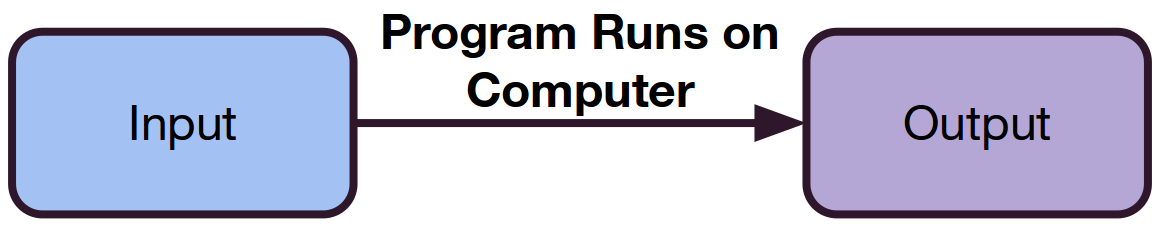
\includegraphics[scale=.2]{program-input-output.png}
\end{center}
\end{frame}

\begin{frame}{What does a programmer do?}
\begin{itemize}
  \item Write human-readable ``source code''
  \item Use another program to interpret that as machine instructions
\end{itemize}
\begin{center}
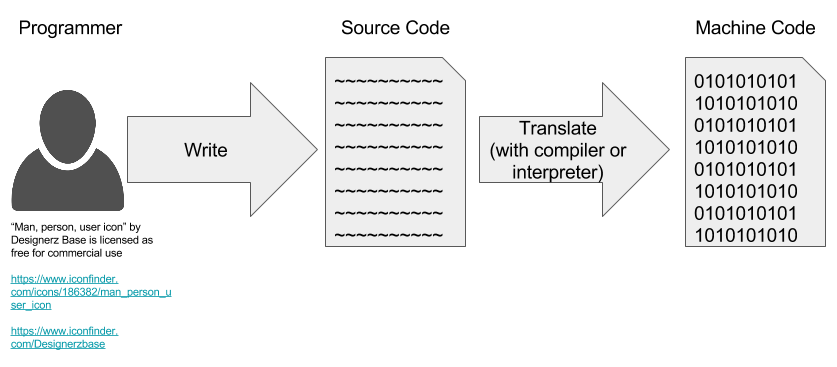
\includegraphics[scale=.34]{human-source-machine.png}
\end{center}
\end{frame}

\begin{frame}{Why do we care about programming?}
  \begin{center}
    
\includegraphics[scale=.30]{logos.png}
  \end{center}
\end{frame}

\begin{frame}{General Programming Steps}
\begin{enumerate}
\item Pick a programming language
\item Write ``source code'' inside a text file
\item Use ``compiler'' or ``interpreter`` to translate source into binary / machine code that is understandable by computers
\item Computer executes code
\end{enumerate}
\begin{center}
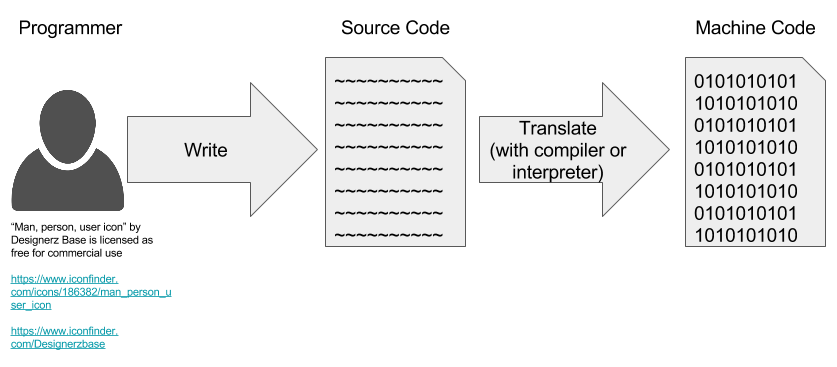
\includegraphics[scale=.34]{human-source-machine.png}
\end{center}
\end{frame}

\begin{frame}{Compilers vs. Interpreters}
\begin{itemize}
\item Compiler outputs machine code into new file
  \begin{itemize}
    \item This binary file is executable
  \end{itemize}
\item Interpreter immediately executes machine code
  \begin{itemize}
    \item The source code file is executable by interpreter
    \item Python is an interpreted language
  \end{itemize}
\end{itemize}
\begin{center}
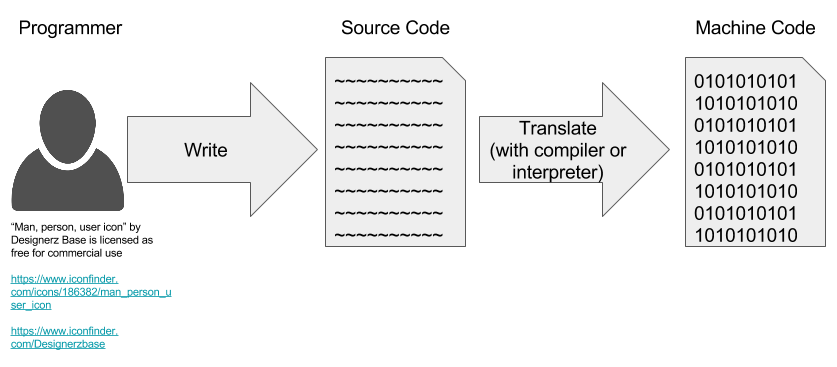
\includegraphics[scale=.34]{human-source-machine.png}
\end{center}
\end{frame}

\begin{frame}{Python Programs}
\begin{itemize}
\item Source code file type is .py
\item Code is written in a text editor
\begin{itemize}
\item Notepad, Notepad++, vim, emacs, gedit, textedit, etc.
\item NOT Word, OpenOffice, LibreOffice
\end{itemize}
\item Use the program called python (the interpreter) to execute code
\item Optionally, an IDE can do both steps
  \begin{itemize}
    \item Python IDLE
    \item Web IDEs, e.g. \url{https://repl.it/languages/python3}
  \end{itemize}
\end{itemize}
\end{frame}

\section{Introduction to Python}

\begin{frame}{Getting Set Up}
Instructions
\begin{enumerate}
  \item Log in to your computer
  \item Open the web browser
  \item Go to \url{https://repl.it/languages/python3}
  \item Type something on line 1 in the left box
  \item Press ``save''
  \item Email the link to yourself, or write it down
\end{enumerate}
\begin{center}
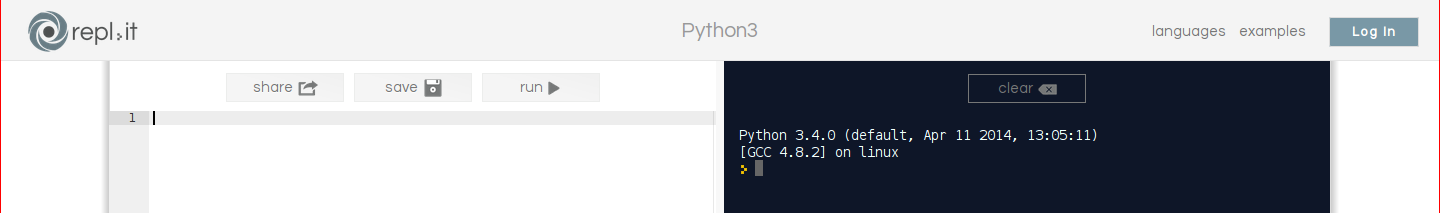
\includegraphics[scale=.2]{repl.png}
\end{center}
\end{frame}

\begin{frame}{repl.it Python Interpreter}
\begin{itemize}
\item Left side is source code, right side is interactive interpreter
\item Type stuff into the right and press ``Enter'' key
\item Type stuff into the left and press ``run'' button
  \begin{itemize}
    \item Don't forget to press ``save'' button periodically
  \end{itemize}
\item In its most basic form, the interpreter acts like a calculator, supporting all basic mathematical operations and orders of operations
\item Of course, Python is infinitely more powerful than this, and we will slowly build up our knowledge of what it can do
\end{itemize}
\begin{center}
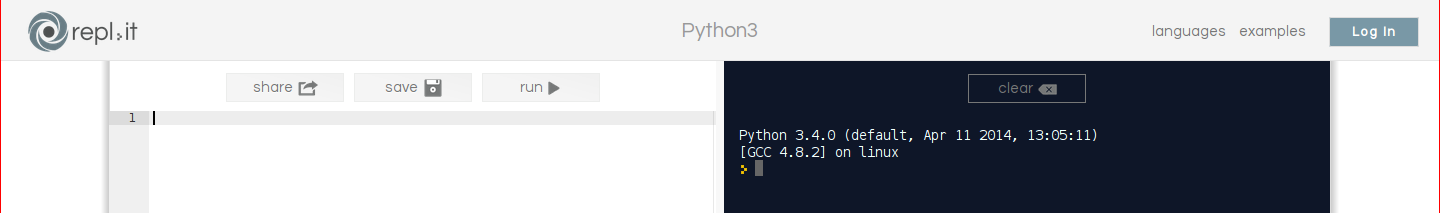
\includegraphics[scale=.2]{repl.png}
\end{center}
\end{frame}

\begin{frame}{Writing and Saving Programs}
\begin{itemize}
\item No code you write into the interpreter on the right is permanent -- it will be lost when you re-run programs from the left
\item For simple one-line statements, use the interpreter on the right to try them out
\item For anything longer, write it into the program window, then ``save'' and ``run''
\end{itemize}
\begin{center}
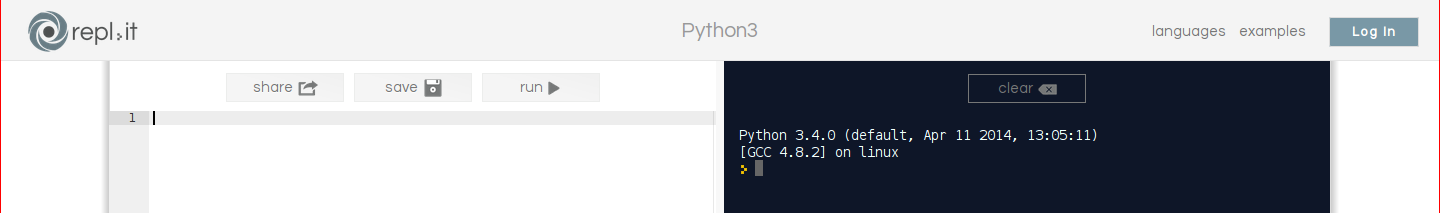
\includegraphics[scale=.2]{repl.png}
\end{center}
\end{frame}

\begin{frame}[fragile]{Hello World! Your First Program!}
\begin{itemize}
\item A programming tradition -- your first program simply outputs the text {\ttfamily Hello World!}
\item ``Output'', in this and most cases, means to write text on the screen
\end{itemize}
Instructions
\begin{enumerate}
  \item Copy this program into the program window on the left
\begin{lstlisting}
# Program: hello.py

print("Hello World!")
\end{lstlisting}
\item Press ``save''
\item Press ``run''
  \end{enumerate}
\end{frame}


\begin{frame}[fragile]{Basic Python syntax}
  \begin{itemize}
    \item Python is CASE SENSITIVE!
  \begin{itemize}
    \item This means that {\ttfamily Print("Hello World!")} is WRONG
  \end{itemize}
\item {\ttfamily \#} starts a comment
  \begin{itemize}
    \item Everything on the line after the {\ttfamily \#} is the comment
    \item Comments have no effect on the program
    \item Use them so others can understand your program
  \end{itemize}
\item {\ttfamily "} starts and ends a string
  \begin{itemize}
    \item A string is a sequence of characters
    \item If you want the quote character, use {\ttfamily \textbackslash"}
      \begin{itemize}
        \item {\ttfamily "\textbackslash"Hello World!\textbackslash""}
          is the string consisting of the characters
        {\ttfamily "Hello World!"}
      \end{itemize}
  \end{itemize}
\item Programs are made up of one-line statements:
\begin{lstlisting}
do_this_first
then_do_that
finally_do_something_else
\end{lstlisting}
  \end{itemize}
\end{frame}

\begin{frame}[fragile]{The {\ttfamily print} Function - Part 1}
  \begin{itemize}
    \item This function is used for outputting text on the screen
    \item {\ttfamily print("Hello World!")} outputs {\ttfamily Hello World!}
    \item {\ttfamily print("text")} outputs {\ttfamily text} (literally)
  \item Don't forget the parentheses and the quotation marks!
  \item The enclosing quotation marks don't show up in the output
  \item After the text, a line break is output
  \item Can include line break in string with {\ttfamily \textbackslash n} character
  \end{itemize}
\end{frame}

\section{Expressions and Variables}

\begin{frame}{So wait, can Python do anything besides print messages?}
  \begin{itemize}
    \item Yes, it can!
    \item Python can calculate the results of expressions
    \item Python can store and manipulate data using variables
  \end{itemize}
\end{frame}

\begin{frame}{Literals}
  \begin{itemize}
    \item The building blocks of expressions
    \item A basic representation of a simple value
    \item Integer literals - {\ttfamily 0}, {\ttfamily 17}, {\ttfamily -10}, etc.
    \item Floating point literals - {\ttfamily 1.0}, {\ttfamily 3.14159}, etc.
    \item String literals - {\ttfamily "Hello World!"}, etc.
    \item Boolean literals - {\ttfamily True}, {\ttfamily False}
  \end{itemize}
\end{frame}

\begin{frame}[fragile]{The {\ttfamily print} Function - Part 2}
  \begin{itemize}
    \item Can be used to print any literal
  \end{itemize}
\begin{lstlisting}
print(17)
print(3.14159)
print("Hello World!")
print(True)
print(False)
\end{lstlisting}
\end{frame}

\begin{frame}{Arithmetic Expressions}
  \begin{center}
  \begin{tabular}{|l|l|l|}\hline
    Addition ({\ttfamily +}) & {\ttfamily 17+5} & {\ttfamily 22} \\\hline
    Subtraction ({\ttfamily -}) & {\ttfamily 17-5} & {\ttfamily 12} \\\hline
    Multiplication ({\ttfamily *}) & {\ttfamily 17*5} & {\ttfamily 85} \\\hline
    Division ({\ttfamily /}) & {\ttfamily 17/5} & {\ttfamily 3.3999999999999999}\\\hline
    Integer Division ({\ttfamily //}) & {\ttfamily 17//5} & {\ttfamily 3}\\\hline
    Modulus ({\ttfamily \%}) & {\ttfamily 17\%5} & {\ttfamily 2} \\\hline
      Parenthesis ({\ttfamily ()}) & {\ttfamily (17+5)*2} & {\ttfamily 44} \\\hline
    Negative ({\ttfamily -}) & {\ttfamily -(17+5)} & {\ttfamily -22} \\\hline
  \end{tabular}
\end{center}
\end{frame}

\begin{frame}[fragile]{The {\ttfamily print} Function - Part 3}
  \begin{itemize}
    \item Can be used to print any expression
\begin{lstlisting}
print(17 + 5)
print(17 - 5)
print(17 % 5)
\end{lstlisting}
\item Can print multiple expressions on one line
\begin{lstlisting}
print("The value of 17 + 5 is", 17 + 5)
\end{lstlisting}
\item Interactive interpreter can print expressions without typing {\ttfamily print}
  \end{itemize}
\end{frame}

\begin{frame}[fragile]{Logical (Boolean) Expressions}
  \begin{center}
  \begin{tabular}{|l|l|l|}\hline
    Equality ({\ttfamily ==}) & {\ttfamily 17==5} & {\ttfamily False} \\\hline
    Inequality ({\ttfamily !=}) & {\ttfamily 17!=5} & {\ttfamily True}\\\hline
    Greater than ({\ttfamily >}) & {\ttfamily 17>5} & {\ttfamily True}\\\hline
    Greater than or equal ({\ttfamily >=}) & {\ttfamily 17>=5} & {\ttfamily True}\\\hline
    Less than ({\ttfamily <}) & {\ttfamily 17<5} & {\ttfamily False}\\\hline
    Less than or equal ({\ttfamily <=}) & {\ttfamily 17<=5} & {\ttfamily False}\\\hline
  \end{tabular}
\end{center}

\begin{lstlisting}
print(17 == 17)
print(17 == 5)
print(17 != 5)
print(17 > 5)
print(17 <= 5)
print(17 == (12 + 5))
print(True == True)
print(True == False)
\end{lstlisting}
\end{frame}

\begin{frame}[fragile]{Variables}
  \begin{itemize}
    \item Can store values into memory locations
    \item Reference this memory with \textbf{variables}
\begin{lstlisting}
variable = expression
\end{lstlisting}
    \item Computes value of \texttt{expression}, and \textbf{assigns} it to \texttt{variable}
\begin{lstlisting}
temperature = 50
average = (17.5 + 73.9) / 2
temperature = temperature - 10
\end{lstlisting}
\item In the last example, the expression value overwrites the old stored value in memory
\item Variable name must start with a letter, consists of letters, numbers, and underscores
  \end{itemize}
\end{frame}

\begin{frame}[fragile]{The {\ttfamily print} Function - Part 4}
  \begin{itemize}
    \item Variables can be used as values, and used in expressions
    \item So \texttt{print} can display stored values
\begin{lstlisting}
temperature = 50
print(temperature)
print(temperature - 10)
\end{lstlisting}
  \end{itemize}
\end{frame}

\begin{frame}[fragile]{User input}
\begin{lstlisting}
name = input("What is your name? ")
print("Your name is", name)

temperature = int(input("What is the temperature? "))
print("That is", temperature - 32, "above freezing")
\end{lstlisting}
\end{frame}

\begin{frame}{Coding Challenge}
  \begin{itemize}
    \item Write code to take two numbers of user input, add them together, and print the result.
    \item Write code to take the temperature in fahrenheit and print it in celsius.
      \begin{itemize}
        \item $C = \displaystyle\frac{F - 32}{1.8}$
      \end{itemize}
  \end{itemize}
\end{frame}

\section{Control Flow}

\begin{frame}[fragile]{Conditional Execution with {\ttfamily if}-statements}
  \begin{itemize}
    \item Execute a block of code only if an expression is \texttt{True}.
\begin{lstlisting}
temperature = int(input("What is the tempurature? "))
print("The temperature is", temperature)
if temperature < 32:
    print("It is below freezing!")
    print("Don't forget to wear your jacket!")
\end{lstlisting}
\item Those messages will only print when the temperature is below 32
\item \texttt{if}, followed by the true/false expression, followed by a colon
\item The conditional block must be indented
  \end{itemize}
\end{frame}

\begin{frame}[fragile]{Conditional Execution with {\ttfamily else}-statements}
  \begin{itemize}
    \item Execute a block of code only if the immediately preceeding \texttt{if}-statement was \texttt{False}
\begin{lstlisting}
temperature = int(input("What is the temperature? "))
print("The temperature is", temperature)
if temperature < 32:
    print("It is below freezing!")
else:
    print("It is", temperature - 32, "degrees above freezing")
\end{lstlisting}
\item \texttt{if}-statement and block, followed by un-indented \texttt{else:} (with colon)
\item The conditional block must be indented
  \end{itemize}
\end{frame}

\pagebreak

\begin{frame}[fragile]{Conditional Execution with {\ttfamily elif}-statements}
  \begin{itemize}
    \item Execute a block of code only if all the immediately preceeding \texttt{if} and \texttt{elif}-statements were \texttt{False}
\begin{lstlisting}
temperature = int(input("What is the temperature? "))
print("The temperature is", temperature)
if temperature < 32:
    print("It is below freezing!")
elif temperature == 32:
    print("We're at the freezing point!")
elif temperature < 100:
    print("It is", temperature - 32, "degrees above freezing")
else:
    print("It is really hot!")
\end{lstlisting}
\item Un-indented \texttt{elif}, followed by the true/false expression, followed by a colon
\item The conditional block must be indented
  \end{itemize}
\end{frame}

\begin{frame}{Coding Challenge Ideas}
  \begin{itemize}
    \item Write code to take two numbers of user input, ask the user for an operation (addition, subtraction, etc.), and print the result.
    \item Write code to take the temperature in fahrenheit and print it in celsius, or do the reverse, depending on user input.
      \begin{itemize}
        \item $C = \displaystyle\frac{F - 32}{1.8}$
        \item $F = (1.8 \times C) + 32$
      \end{itemize}
    \item Write a basic game, such as rock-paper-scissors.
  \end{itemize}
\end{frame}

\begin{frame}{More Learning Resources}
  \begin{itemize}
    \item \url{https://docs.python.org/3/}
    \item \url{https://docs.python.org/3/tutorial/index.html}
    \item \url{https://www.python.org/downloads/release/python-350/}
    \item \url{https://en.wikibooks.org/wiki/Python\_Programming}
    \item \url{http://www.diveintopython3.net/}
    \item \url{http://www.codecademy.com/en/tracks/python}
    \item \url{https://wiki.python.org/moin/PythonBooks}
  \end{itemize}
\end{frame}

\end{document}
